% !TeX spellcheck = pt_BR
\chapter{Desenvolvimento}
\label{chap:desen_test}
\begin{flushright}
	"Insanidade é continuar fazendo sempre as mesmas coisas, \\ 
	esperando resultados diferentes." \\
	\ \\
	(Albert Einstein)
\end{flushright}

Durante cada uma das etapas da metodologia, uma série de tarefas foram elaboradas e cumpridas. Este capítulo irá tratar do desenvolvimento de cada dessas etapas de acordo com a metodologia utilizada na realização deste projeto.

\section{Etapa Conceitual}
\subsection{Levantamento de Requisitos}
O primeiro passo para o desenvolvimento do projeto foi o de reunir todos os requisitos que deveriam ser cumpridos pelas entregas. A partir de conversas com o cliente, pode-se levantar alguns requisitos iniciais.

As funcionalidades esperadas pelo cliente foram um kit físico dividido em módulos integrados e complementares. O kit deveria culminar na montagem de um robô com movimentação cinemática e funcionalidade de visão computacional utilizando uma câmera RGB.
 
Além disso o cliente esperava também tutoriais online abrigados em domínio aberto, escritos em linguagem simplificada, abordando conceitos introdutórios da robótica, como por exemplo: O que é um robô, partes de um robô, funcionalidades de um robô completo, áreas da robótica e suas funcionalidades, atuação e movimentação diferencial, introdução a visão computacional e integração com a movimentação.

Um outro ponto exigido pelo cliente foi a utilização de desafios ao longo do desenvolvimento através do kit, com o intuito de manter o estudante engajado e interessado durante a sua interação com o kit.

Por fim o cliente pediu ainda que fossem abordados conceitos de ferramentas utilizadas profissionalmente, em específico o framework ROS, alguma linguagem de programação e alguma biblioteca para auxilio de aprendizado na questão da visão computacional.

\subsection{Estudo do Estado da Arte}
De posse dos requisitos do projeto, o passo seguinte foi a realização de uma pesquisa sobre as principais tecnologias e projetos já existentes no mercado, tanto nacional quanto internacional, que cumpriam parcialmente ou totalmente com os requisitos levantados. Neste estudo, os principais envolvidos encontrados foram: Modelix Robotics, Robocore, Nvidia, Mini Maker, Gogo Board, Lego e Vex Robotics.
A figura 4.1 apresenta o levantamento das principais marcas do mercado, com suas referentes características quanto a metodologia de aprendizado, disponibilidade e presença de framework.

\begin{figure}[h!]					
	\centering					
	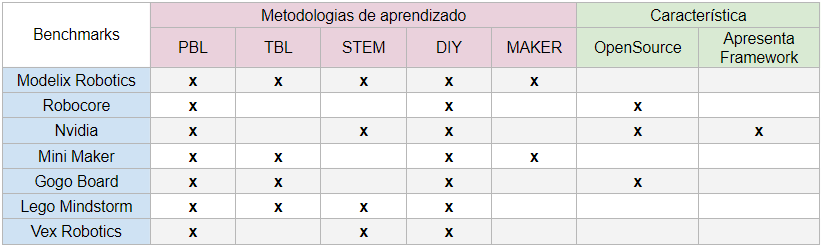
\includegraphics[width=1.0\textwidth]{figura1tabelametod.png}			
	\caption{Características analisadas no SOTA}		
	\label{img:sotabru}	
	\source{Autores, 2019}		
\end{figure}

Fazendo uma análise quanto a hardware e especificações, observou-se que são opensource apenas os prejetos da Robocore, Gogo Board e Nvidia, sendo este último o único a apresentar framework.


\subsection{Estudo das Metodologias de Ensino}
	
Através do estudo do estado da arte, foi notado que há uma certa variabilidade de métodos de ensino aplicados em cada benchmark, o que levantou a necessidade de um aprofundamento no campo pedagógico com estudo detalhado quanto aos principais movimentos, filosofias e metodologias de ensino aplicadas nos modelos de referência mundiais no ensino de robótica. 

Primeiramente, foram analisadas as características do público alvo, com visão direcionada para as principais dificuldades e barreiras que as metodologias atuais de ensino possuem para se adequar ao perfil desse público. Notou-se que atualmente as pessoas acima de 12 anos estão o tempo inteiro conectadas à internet, recebem enorme quantidade de informações e não possuem mais paciência para aulas expositivas, havendo preferência por entretenimento através de games, redes sociais e outras ferramentas ao invés do estudo de ciências e tecnologias. Sendo assim, foi compreendido que é necessário transformar o aprendizado de robótica em algo divertido e prático, adequando-se ao perfil dinâmico dos alunos modernos e fazendo da robótica um meio prazeroso de entretenimento para atrair entusiastas.

Foi, então, realizada uma busca das principais e mais eficientes didáticas de ensino aplicadas na aprendizagem de robótica ao redor do mundo. Decidiu-se incorporar ao projeto as seguintes filosofias, movimentos e metodologias com o intuito de adequar-se aos padrões mundiais de ensino de robótica e ao perfil dos alunos, facilitando e otimizando o aprendizado do público alvo:
\begin{itemize}
	\item aprendizagem baseada em projetos e colaboração: através de um kit modularizado com etapas progressivas que estimulam o empenho e a zona de desenvolvimento proximal para solucionar problemas e exploram o potencial de aprendizado enquanto o aluno busca conquistar o resultado final;
	\item movimento STEM: por meio de linguagem simples, clara, interessante e objetiva, de design atrativo e desafios divertidos que desmistificam tabus quanto às dificuldades da área de robótica e atraem a atenção do público;
	\item metodologia Do-It-Yourself aliada à filosofia Maker: estimulando e permitindo que o aluno faça o próprio projeto sem a necessidade de ambiente acadêmico/escolar por meio de peças disponíveis para produção por manufatura aditiva em impressoras 3d, conteúdo opensource e hardwares genéricos.
\end{itemize}

Sendo definidas as metodologias a serem aplicadas, tornou-se possível entender e adotar uma série de cuidados necessários para adequar o desenvolvimento do projeto às necessidades do público alvo.

\section{Projeto Detalhado}
\subsection{Definição}
Após a realização das etapas descritas anteriormente, pôde-se de fato escrever uma solução proposta. A solução proposta foi dividida em duas partes, o Kit Físico e os Tutoriais, como descrito a seguir.

Kit Físico: Utilização da Raspberry Pi como controlador central, utilização dos dynamixels mx-28 como atuadores, kit modulado com módulos integrados e sequenciais para montagem de um robô reconhecedor de marcos fiduciais. A finalização do Kit culminará em um robô com movimentação diferencial e capacidade de visão com a utilização de uma câmera RGB.

Tutoriais: Linguagem simples e acessível, metodologia intuitiva, presença de desafios.
Conteúdos a serem abordados: Breve histórico da robótica, partes de um robô, funcionalidades encontradas em robôs completos, introdução a áreas da robótica, abordagem prática do framework ROS em compatibilidade com a Raspberry Pi, abordagem prática de conceitos de programação em Python com a utilização de programas modelos acompanhados de tutoriais de mudança e proposição de desafios,
programação de atuação dos servos para movimentação diferencial simples, abordando conceitos facilitados de cinemática diferencial e seu funcionamento. Introdução à visão computacional com introdução a biblioteca do OpenCV e tratamentos simples de imagens.
Implementação de uma integração da movimentação com a visão computacional.
\subsection{Planejamento}

\section{Confecção}
\subsection{Protótipo Físico}
O Kit Físico foi pensado para ser uma forma de concretização dos conceitos abstratos que são abordados ao longo dos tutoriais. A ideia foi de criar um robô que funcionaria a partir de movimentação diferencial e que fosse capaz de trabalhar com os conceitos de cinematica e visão computacional em conjunto.

De forma a otimizar o design do robô, algumas considerações iniciais foram levantadas anteriormente ao inicio do design:

\begin{itemize}
	\item O robô deve ser compacto;
	\item O robô deve ser apresentar boa resistência mecânica em geral;
	\item O robô será majoritariamente fabricado por manufatura aditiva;
	\item O robô deve ser composto por peças para montagem gradual;
\end{itemize}
A partir destes detalhes iniciou-se o design do robô. Utilizou-se o software SOLIDWORKS 2019 para criar o design de forma interativa. As geometrias buscadas tem características modernas e foram pensadas também para serem eficazes no que concerne a fabricação por manufatura aditiva.

Tomando como base o componente de maior peso e volume do sistema, a bateria, foi criada a peça "Chassi 1" para mantê-la na região central e deixar o motor equilibrado com um centro de gravidade centralizado e baixo. A imagem~\ref{fig:chassi_1} abaixo representa essa peça.

\begin{figure}[h!]
	\centering
	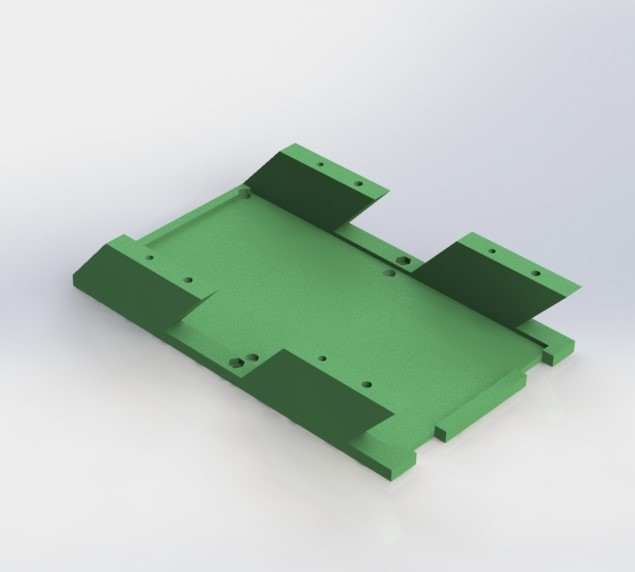
\includegraphics[width=10cm, height=8cm, angle=0]{chassi_1.jpg}\\
	\caption{Peça Chassi 1 \\ Fonte: Autores, 2019}
	\label{fig:chassi_1}
\end{figure}

O rebaixo feito no principal chassi foi feito para manter a bateria encaixada e evitar seu movimento durante o deslocamento do sistema. Além disso, em diversas partes do design do robô, utilizou-se o conceito de Poka Yoke para que o encaixe das peças seja intuitivo e erros sejam prevenidos no momento da montagem. Isso pode ser visto nos quatro furos cilíndricos no chassi que servirão unicamente para encaixar os pinos de peças que se encaixam ao chassi. Na parte frontal do Chassi também existem entradas para que o Chassi 2 se acople a ele.

O segundo componente a ser criado foi o suporte do Dynamixel, que será responsável por fixar os servomotores ao chassi principal. Este componente é simples e foi feito para se encaixar perfeitamente no Dynamixel, com furo para passagem do eixo e pinos
para encaixe, como demonstrado na figura~\ref{fig:suport_dyn} abaixo.

\begin{figure}[h!]
	\centering
	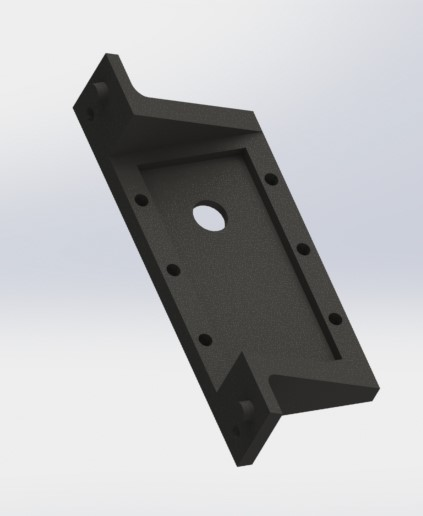
\includegraphics[width=7cm, height=8cm, angle=0]{suport_dyn.jpg}\\
	\caption{Peça Suporte Dynamixel \\ Fonte: Autores, 2019}
	\label{fig:suport_dyn}
\end{figure}

Em seguida, foram criadas as rodas traseiras do robô, como demonstradas na figura ~\ref{fig:roda_} abaixo, responsáveis por transmitir a tração dos motores e movimentar a estrutura. Sua geometria foi pensada de forma em que sejam encaixadas no flange do Dynamixel com quatro parafusos para a fixação. Um parafuso adicional será utilizado para conectar a roda ao eixo.

\begin{figure}[h!]
	\centering
	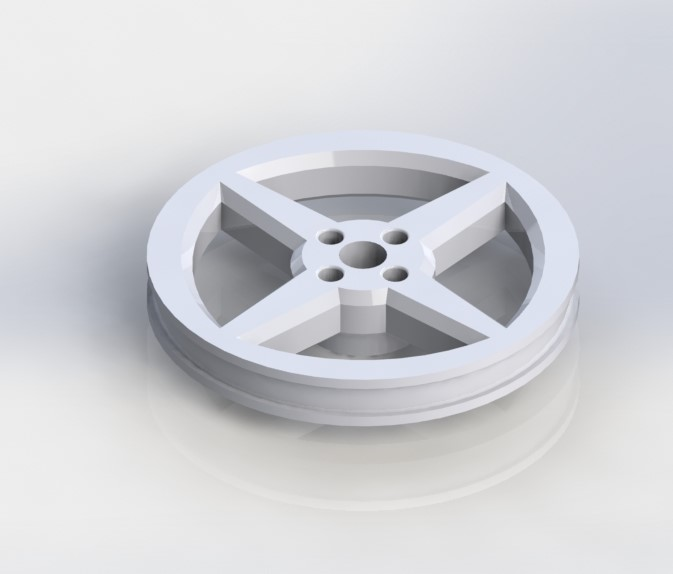
\includegraphics[width=6cm, height=6cm, angle=0]{roda_.jpg}\\
	\caption{Peça Roda Traseira \\ Fonte: Autores, 2019}
	\label{fig:roda_}
\end{figure}

Com as duas rodas traseiras sendo as únicas responsáveis pela tração, foi necessário criar um sistema de roda boba na parte frontal do robô, para que este consiga se deslocar em qualquer direção com a devida sustentação. Para isso, foi criado uma peça
a ser fixada no chassi principal que terá a função de segurar uma esfera, que servirá de roda boba. Uma peça menor será responsável por manter a esfera sempre em contato com o chão, empurrando-a de cima para baixo. Essas peças estão demonstradas na figura~\ref{fig:roda_boba} abaixo, e o esquema para montar esse subsistema está demonstrado na imagem~\ref{fig:roda_boba_montado} abaixo.

\begin{figure}[h!]
	\centering
	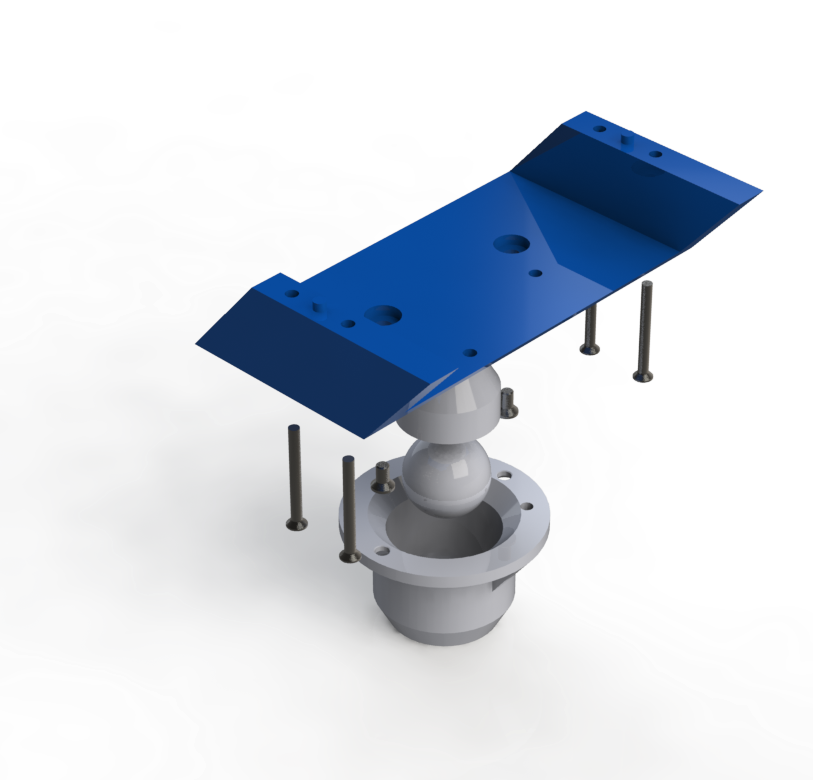
\includegraphics[width=8cm, height=7.5cm, angle=0]{roda_boba.png}\\
	\caption{Peças da Roda Boba \\ Fonte: Autores, 2019}
	\label{fig:roda_boba}
\end{figure}

\begin{figure}[h!]
	\centering
	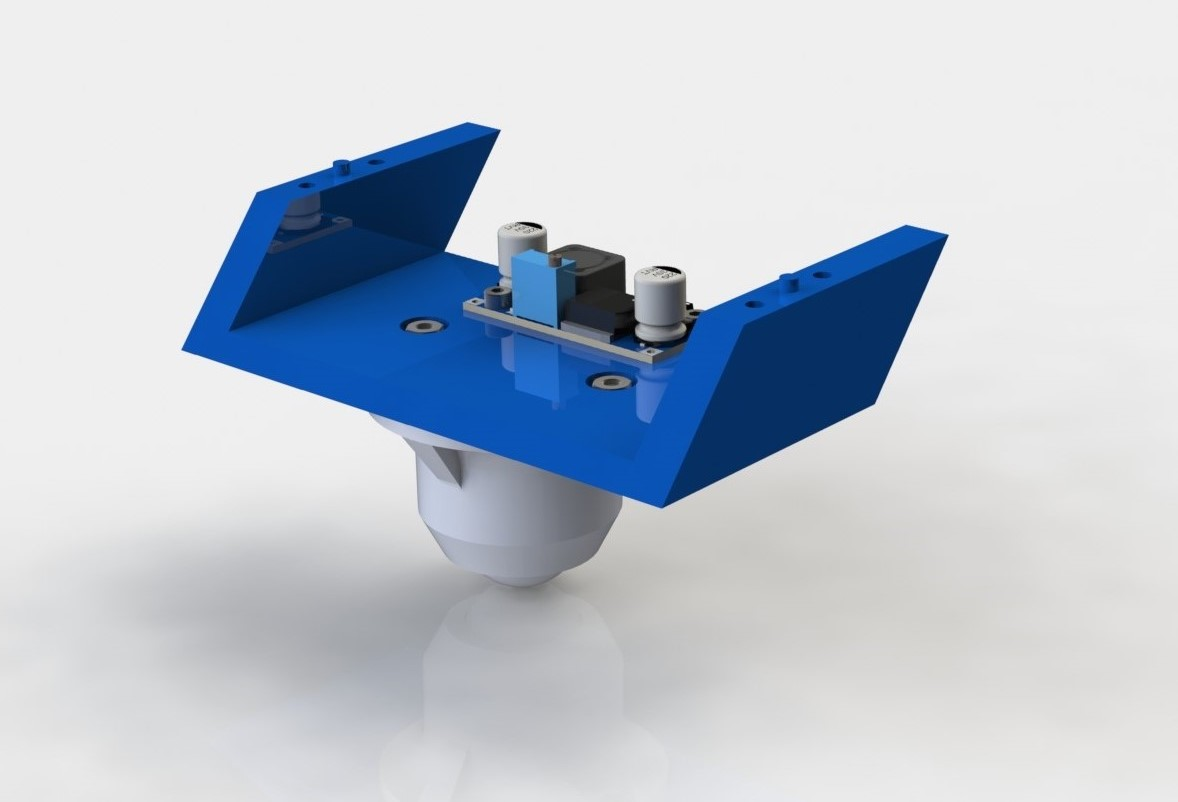
\includegraphics[width=9cm, height=7cm, angle=0]{roda_boba_montado.jpg}\\
	\caption{Montagem da Roda Boba \\ Fonte: Autores, 2019}
	\label{fig:roda_boba_montado}
\end{figure}

Todo esse conjunto será fixado primeiramente no Chassi 3, que tem como função conectar o conjunto da roda boba ao chassi principal e servir de base para o primeiro conversor DC-DC. O conversor DC-DC tem a função de regular a tensão da bateria que sai a 14,4V e precisa chegar ao Raspberry com 5V.

Com a parte inferior do robô finalizada, deu-se início a construção da parte superior, onde fica o cérebro do robô, o Raspberry Pi. Para servir de base para o Raspberry e de cobertura para a bateria, o Chassi 2 foi criado, como mostrado na figura~\ref{fig:chassi_2}

\begin{figure}[h!]
	\centering
	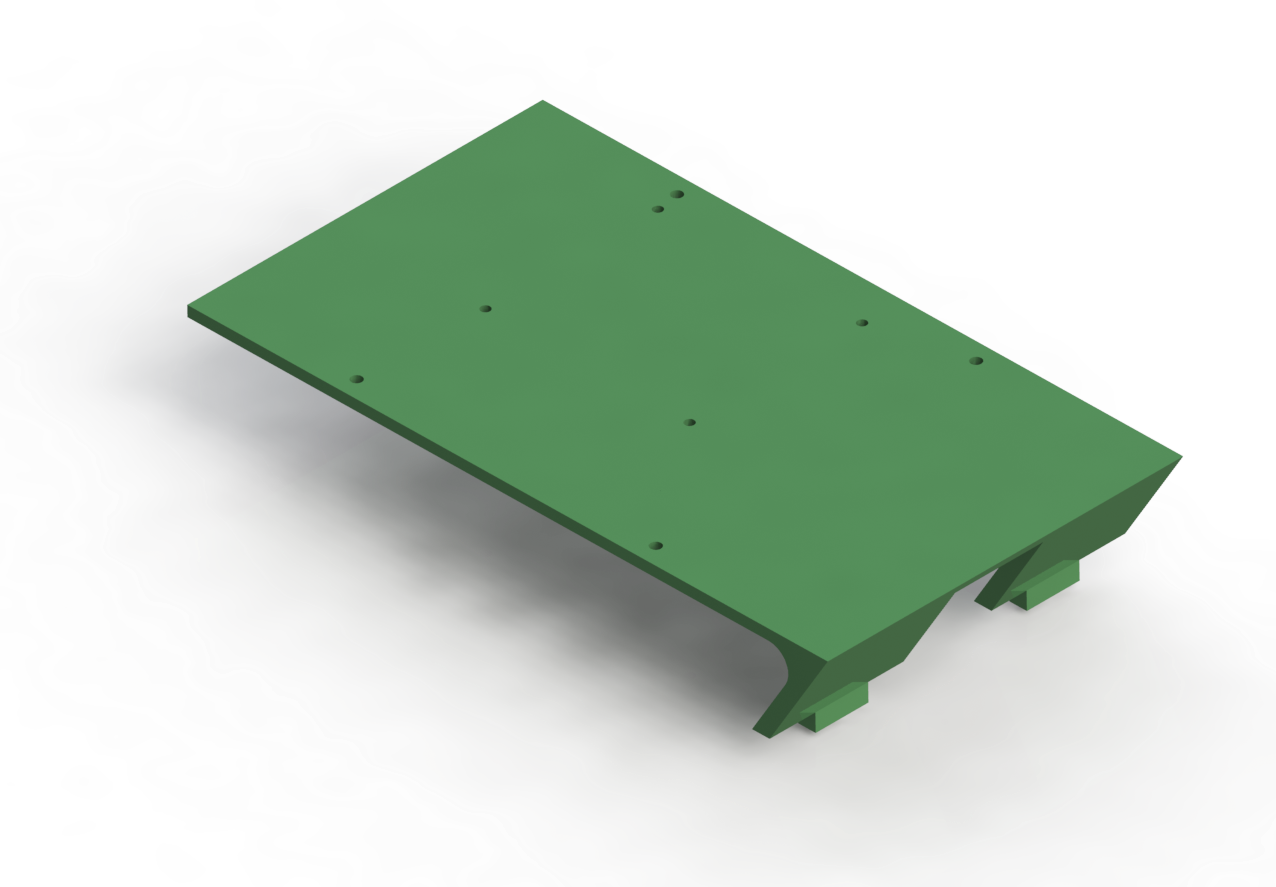
\includegraphics[width=9cm, height=7cm, angle=0]{chassi_2.png}\\
	\caption{Peça Chassi 2 \\ Fonte: Autores, 2019}
	\label{fig:chassi_2}
\end{figure}

Foram alocados quatro furos para segurar a Raspberry, dois furos para o segundo conversor DC-DC e mais quatro furos para a fixação no chassi principal. O Raspberry Pi funciona como um mini computador, o qual terá os códigos e informações necessárias para acionar os
motores.

Por fim, uma capa foi criada para proteger a Raspberry e o conversor da parte superior, além de dar um aspecto moderno ao robô, com linhas diagonais simulando uma seta para frente, como demonstrado na figura~\ref{fig:capa_learn} abaixo. Em frente a capa foi deixado um espaço para a Webcam, que fará as filmagens e auxiliará o sistema a interpretar as imagens com a visão computacional. Ao lado foi feito um corte para permitir a passagem dos conectores HDMI e Micro USB ao Raspberry Pi.

\begin{figure}[h!]
	\centering
	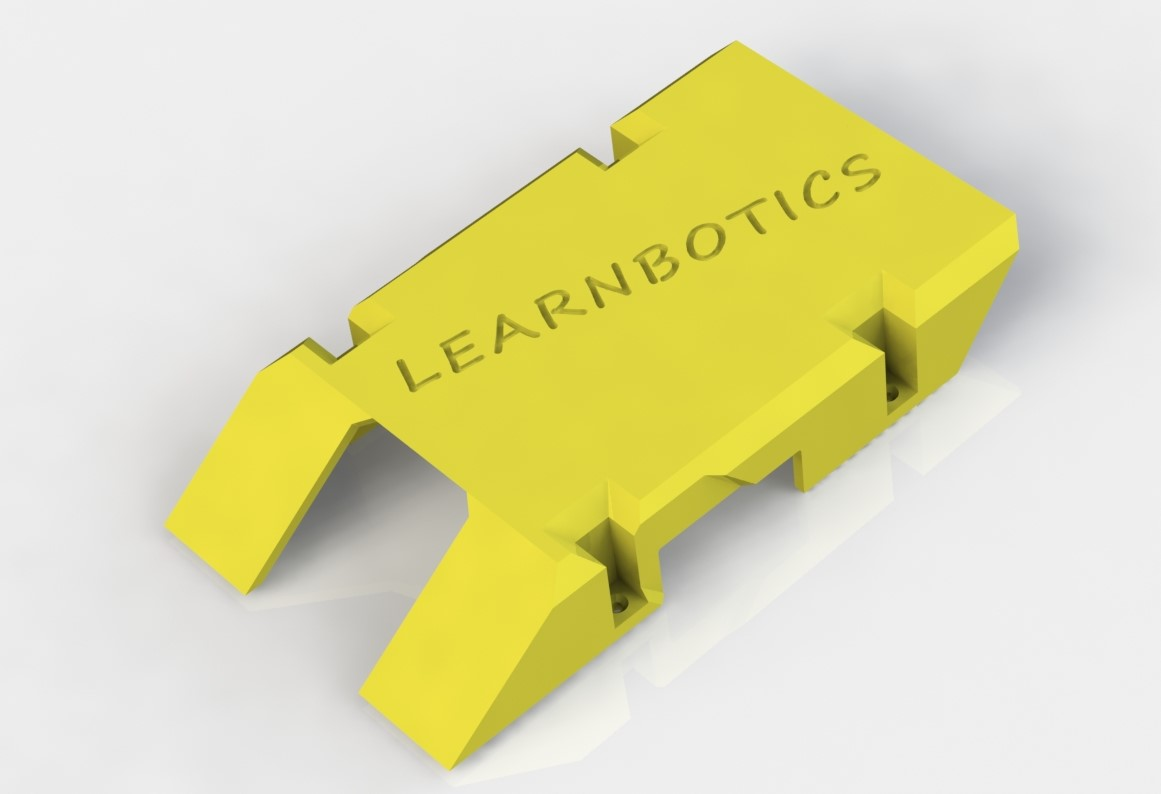
\includegraphics[width=11cm, height=7cm, angle=0]{capa_learn.jpg}\\
	\caption{Peça Capa Superior \\ Fonte: Autores, 2019}
	\label{fig:capa_learn}
\end{figure}

Como mencionado anteriormente, o robô foi pensado para que em sua grande maioria, com exceção de componentes já prontos e peças de fixação como parafusos e porcas, fosse fabricado através de manufatura aditiva.

Essa decisão se justifica devido ao fato de que o proposto por essa abordagem de ensino tem como finalidade ser democrática e abrangente para diversos públicos. A utilização de Impressoras 3D para fabricação das peças do robô é fundamental para essa questão, uma vez que possibilita que qualquer pessoa que possua uma impressora, seja capaz de fabricar as peças e utilizar o kit.

Após fabricação concluída, disponibilização dos componentes de fixação, disponibilização dos componentes eletrônicos e dos dispositivos utilizados no kit, todos os componentes que se tem no robô estão listados abaixo:
\begin{itemize}
	\item 2 Servomotores Dynamixel MX-28
	\item 2 Chassis (1 e 2)
	\item 1 Capa do robô
	\item 2 Suporte para os Servomotores
	\item 2 Rodas traseiras
	\item 2 Flanges Dynamixel
	\item 1 Esfera de 15mm
	\item 1 "EmpurraEsfera"
	\item 1 "SeguraEsfera"
	\item 1 Raspberry Pi 3 b+
	\item 1 Webcam
	\item 1 Bateria Inspired Energy
	\item 2 Conversores DC-DC
	\item 12 Porcas M2.5
	\item 2 Porcas M3
	\item 16 Parafusos de cabeça escareada M2.5 de 12mm
	\item 4 Parafusos de cabeça escareada M2.5 de 25mm
	\item 8 Parafusos Allen de cabeça cilíndrica 3-48 1/2"
	\item 2 Parafusos Allen de cabeça cilíndrica 3-48 7/16"
	\item 2 Parafusos Allen de cabeça escareada M3 de 6mm
	\item 8 Parafusos Allen de cabeça cilíndrica M2.5 de 4mm
\end{itemize}
Com todos os componentes em mãos, o estudante pode proceder para a montagem acompanhando o passo a passo disponibilizado no tutorial de montagem do robô. O resultado da montagem do robô pode ser visualizado na figura ~\ref{fig:learnbotics_rend} a seguir.
\begin{figure}[h!]
	\centering
	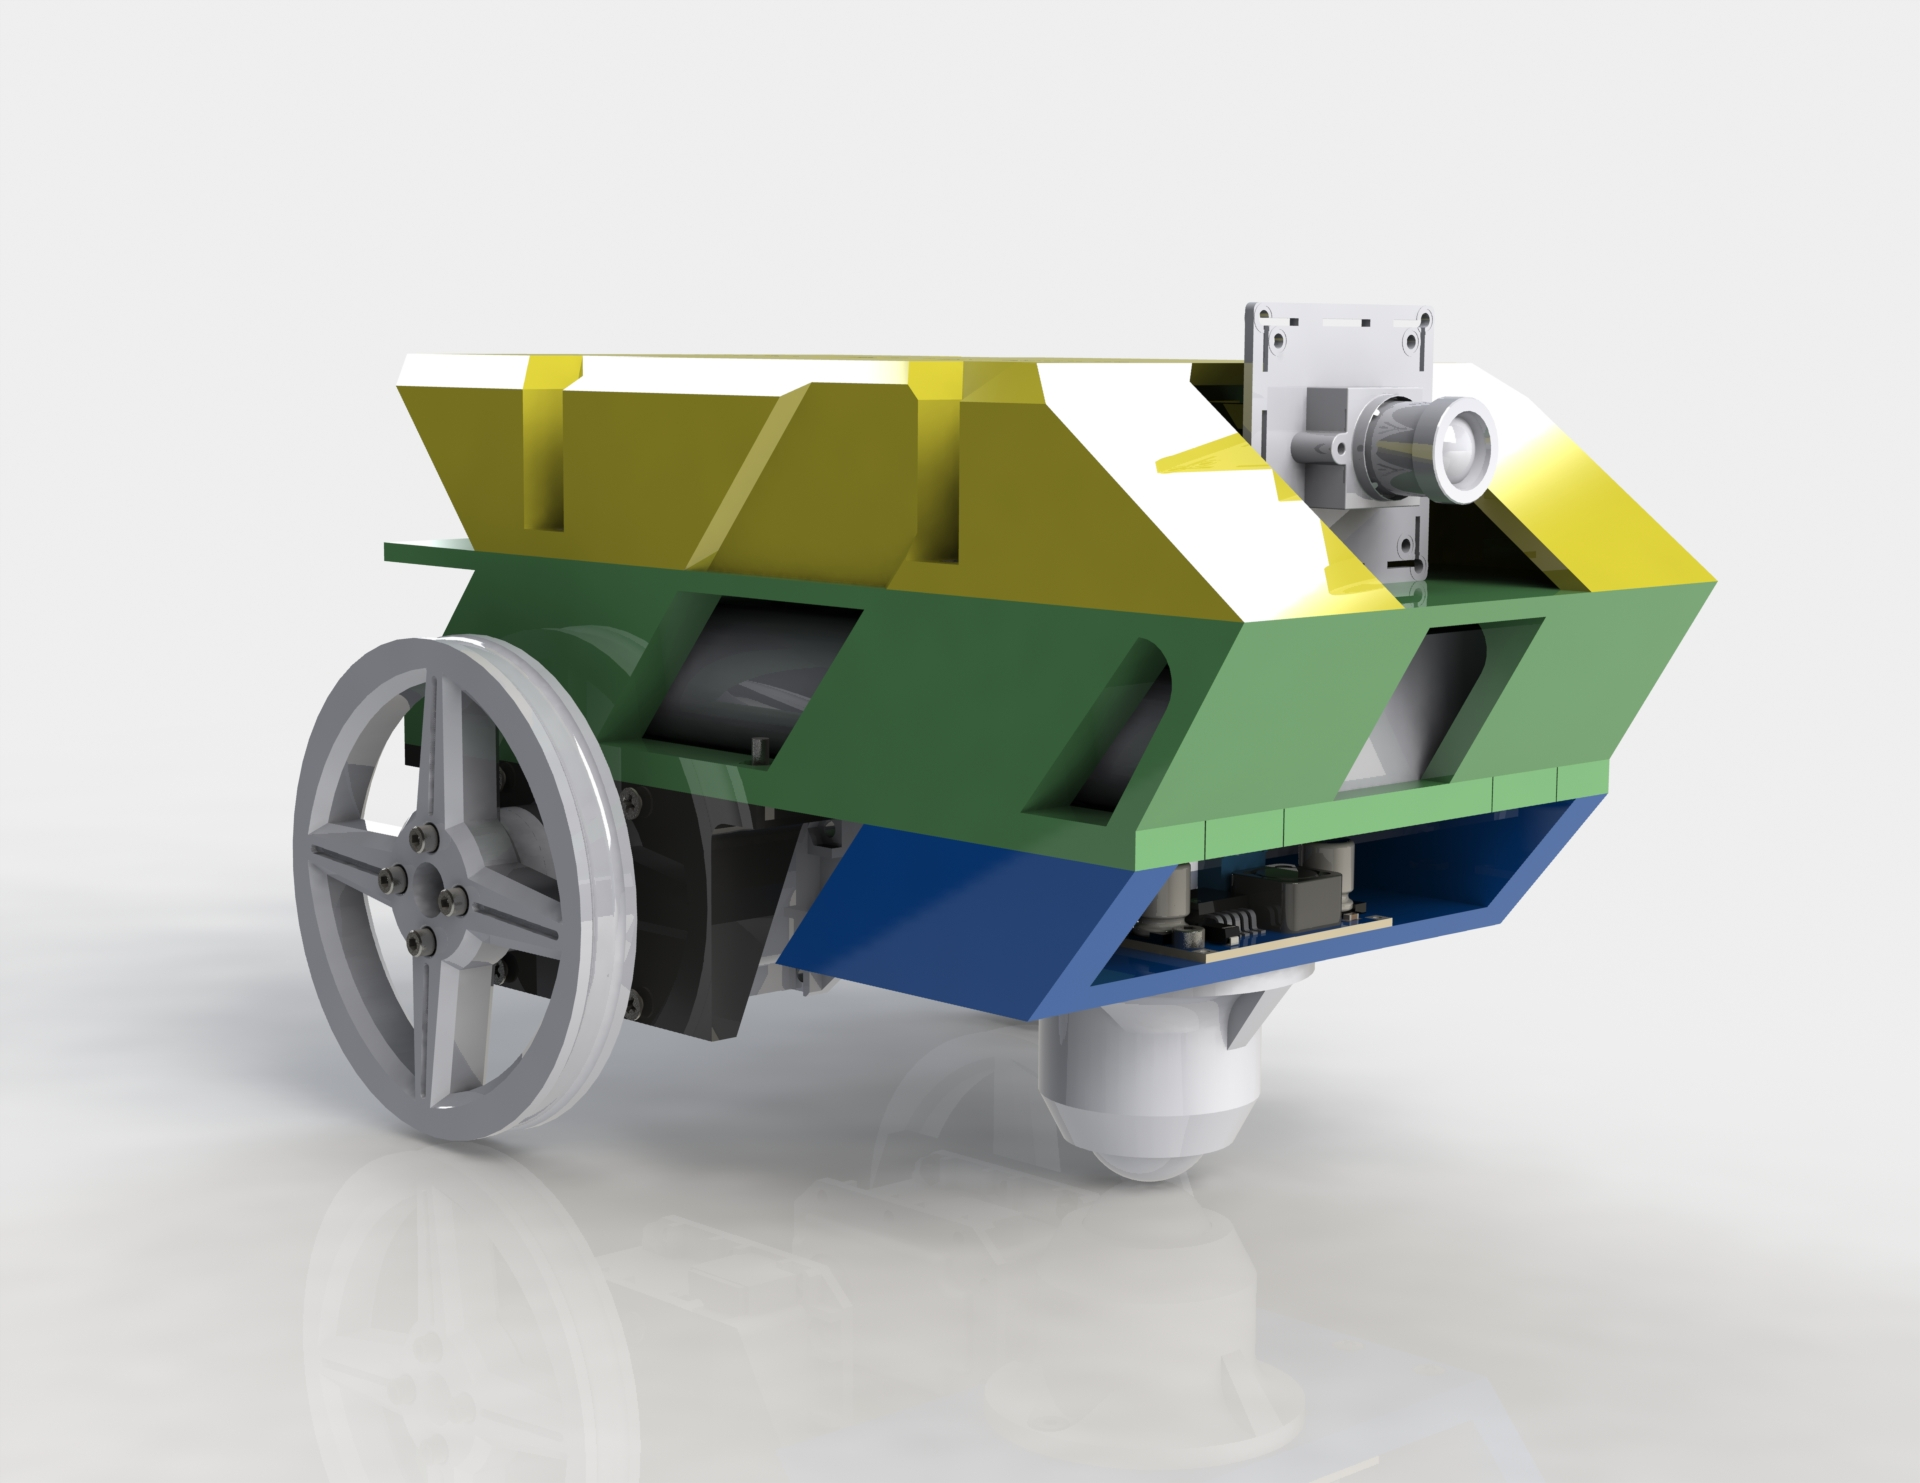
\includegraphics[width=12cm, height=10cm, angle=0]{learnbotics_rend.jpg}\\
	\caption{Robô Completo \\ Fonte: Autores, 2019}
	\label{fig:learnbotics_rend}
\end{figure}

\subsection{Material Escrito}
De forma a melhor organizar a elaboração do conteúdo dos tutoriais, uma divisão dos mesmos foi feita de acordo com o assunto abordado, ocasionando assim uma menor abrangência de assuntos a serem pesquisados, de conteúdos a serem concentrados e de novas interpretações a serem elaboradas.

A primeira sessão dos tutoriais conta com os tutoriais de conceitos básicos, e seguiu o processo de elaboração como detalhado a seguir.

Para contextualizar o estudante sobre o que será aprendido no decorrer do kit foi feita uma breve introdução sobre a história dos robôs, de como surgiu a palavra robô até a construção do primeiro sistema robótico, o UNIMATE. Além desta introdução também foi introduzido, de forma simplificada, o funcionamento de um sistema robótico.

Antes do estudante se aprofundar nos estudos da robótica, deverá ter noções básicas acerca dos conceitos a ser apresentados no decorrer do kit. Para isto, foram apresentados os conceitos superficiais da robótica atual: percepção, visão computacional e navegação e mapeamento. Desta forma, já estará familiarizado com os conceitos quando forem aprofundados.

Um outro conceito básico que o estudante deve assimilar é o conceito de algoritimo e programação. Pois a comunicação entre os computadores e os seres humanos se dá através de linguagens de programação, que se utilizam do conceito de algoritmo para desenvolver suas lógicas. Já os robôs são mecanismos gerenciados por sistemas computacionais para resolução de problemas - auxiliam os seres humanos em tarefas complexas ou repetitivas. Portanto é essencial que o aluno desenvolva conhecimentos sobre algoritmo para que assim seja possível alcançar, através dos algoritmos, o desenvolvimento de comandos que o robô executará.

Após essa parte, deu-se início a confecção dos tutoriais sobre conceitos técnicos que o aluno deverá aprender. O primeiro passo, respeito a modularização proposta, foi falar sobre atuação.

Para que o estudante possa compreender de uma forma mais aprofundada o que está fazendo, antes de começar a mexer com os Dynamixels, uma pequena introdução a atuação foi elaborada.

Essa Introdução trata de uma forma simplificada do conceito de atuadores, de tipos de atuadores, de conversão de energia, e apresenta exemplos cotidianos de atuadores explicando seu funcionamento e aprofundando um pouco mais os conceitos de conversão de energia. \cite{tutAtua}

Após ter tido contato com o conceito de atuadores, o estudante irá encontrar também um tutorial que faz uma introdução aos servo-motores inteligentes Dynamixel$^{TM}$.

Neste tutorial são apresentados os servo-motores inteligentes, suas diferenças para servo-motores comuns, suas vantagens sobre os comuns, qual o papel destes servo-motores no robô e no kit físico e mais precisamente porquê escolhemos utilizar os Dynamixels, e não servo-motores comuns. \cite{tutDyna}

Após ter sido apresentado aos dynamixels e ter tido condições de ligá-los, o próximo passo para começar a utilizá-los depende antes dos conceitos e da utilização do framework ROS.

Tendo em vista a ídeia de apresentar ao estudante ferramentas que são de fato utilizadas por profissionais da área, buscamos realizar um material completo sobre as partes iniciais de utilização do framework ROS.

Devido ao nível de conteúdo que é abordado nos tutoriais nativos do ROS, foi feita uma análise de relevância dos conteúdos e uma reescrita completa do conteúdo abordado, trazendo novas abordagens para passar esse conhecimento para o estudante.

Este tutorial foi dividido em quatro partes, sendo elas, em ordem:
\begin{itemize}
	\item Introdução: O que é o ROS e como funciona;
	\item Conceitos Básicos: Apresentação de terminologia e conceitos base utilizados pela comunidade do ROS.
	\item Entendendo como Funciona o ROS: Apresentação de conteúdo novo que foi elaborado com base em analogias para facilitar o entendimento do estudante sobre a ferramenta.
	\item Tutoriais do ROS: Os Tutoriais de fato, onde o aluno irá aprender a configurar e utilizar o ROS.
\end{itemize}

A parte quatro, ou parte dos tutoriais de fato, aborda todos os conceitos de nível iniciante apresentados nos tutoriais oficiais do ROS. Porém estes conceitos foram demonstrados de forma mais simplificada, com linguagem mais simples e de forma acompanhada passo a passo para uma melhor assimilação do estudante.

Todos os tutoriais foram traduzidos do inglês para o poruguês, visando assim facilitar o acesso à uma amostragem maior de estudantes. \cite{tutROS}

Após ter obtido o conhecimento básico sobre o framework ROS em associação com o que foi passado nos tutoriais sobre os servo-motores a sequência foi de apresentar os tutoriais sobre os scripts de cinemática utilizados.

Nesta parte dos tutoriais o estudante terá acesso ao programa que fará com que o seu robô ande. Além disso será ensinado também como o estudante deve proceder para que transforme seu código em um código executável e para rodá-lo.

De forma a estimular o estudante, uma análise mais minusciosa do código, com comentários parte a parte também foi feita. A partir da explicação do que os comandos do programa fazem o estudante terá condições de alterá-lo para concluir etapas e descobrir coisas por si só.

Para finalizar, o tutorial apresenta um desafio para que o estudante de fato assimile o que lhe está sendo proposto, alterando o código e vendo na prática o que isso ocasiona. \cite{tutCinemat}

Após concluída toda a seção de movimentação do robô, passou-se a elaborar a sessão que trata dos conceitos e utilização da visão computacional. 

Para o ensino de visão computacional apresentado na wiki do Github do Learnbotics \cite{wikilearn}, foi-se pensado na explanação dos conceitos de forma branda e intuitiva, já que, conceitos que se relacionam com visão computacional podem torna-se um tanto rebuscados quando buscados na bibliografia. Os principais conceitos abordados foram:
\begin{itemize}
	\item O uso da visão computacional;
	\item Características  (\textit{Features})
	\item Cantos, arestas e linhas (\textit{Corners,edges e lines})
	\item OpenCV
	\item Segmentação e identificação de cores
	\item Marcos fiduciais
	\item Pose
	\item Identificação de arucos
	
\end{itemize}

Os conceitos apresentados são suficientes para o objetivo do trabalho. Após a construção destes textos na wiki \cite{tutVis}, a equipe disponibilizou para uma pequena amostragem de pessoas a fim de receber feedbacks. Dentro desta amostra, haviam pessoas que trabalhavam com o assunto, que conheciam o uso e que não havia conhecimento prévio de visão computacional. Os principais tópicos abordados nos feedbacks foram:

\begin{itemize}
	\item Boa didática;
	\item Maior número de exemplos nos conteúdos abordados
	\item Conceitos apresentados de forma correta e correlacionando com exemplos do cotidiano
	\item Pequenos erros de digitação e ortografia
\end{itemize}

Os feedbacks, em resumo, foram positivos dos três grupos, tendo como consequência o auxílio a equipe a alcançar de forma satisfatória o intuito de explanar satisfatoriamente a área da visão computacional.

Como previamente abordado neste trabalho, um dos métodos de ensino proposto pela equipe foi a apresentação de desafios. Nos tutoriais foram apresentados os conceitos atrelados à desafios. Estes desafios tinham como intuito a validação dos temas abordados. Um exemplo de desafio proposto, foi o de segmentação de cores, no qual o usuário deve segmentar a cor azul. Para que o aluno conseguisse ter êxito neste desafio, a equipe apresentou  um algoritmo de segmentação da cor vermelha, previamente testado. O resultado pode ser observado na figura \ref{fig:vermelho} abaixo:

\begin{figure}[H]
	\centering
	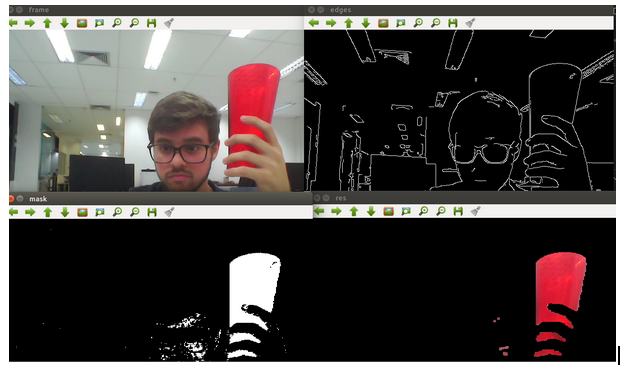
\includegraphics[scale=0.75, angle=0]{Figures/vermelho.png}
	\caption{Exemplo de segmentação de cores}
	\label{fig:vermelho}
	\source{Autores, 2019}
\end{figure}

O último passo foi a elaboração de um tutorial de montagem do robô, uma vez que não é interessante apenas fornecer as peças para o aluno e sua ordem de montagem, mas também fornecer uma linha de raciocínio para que o mesmo não se frustre diante da montagem do robô. O tutorial conta ainda com a sugestão das ferramentas que devem ser utilizadas juntamente com as peças específicas.

\subsection{Desafios}
Ao longo do desenvolvimento dos tutoriais, efetuou-se esforços para pensar e configurar desafios que serviriam como marcos para cada etapa em que o estudante conseguisse avançar. 

Nos tutorias de cinemática por exemplo, após o estudante ter contato com os scripts que fazem seus motores andarem para frente, foi proposto como desafio que o estudante fizesse com que os motores fizessem o robô dar uma meia-volta. Esses desafios foram pensados de uma forma que caso o estudante tenha obtido um certo nível básico de proficiência a partir das análises dos programas modelos, ele conseguiria realizá-los com uma simples mudança no código.

Um outro exemplo desses desafios é o desafio contido na parte introdutória de visão computacional. Foi apresentado para o aluno como seria um script para isolamento e segmentação da cor vermelha em uma imagem, e o desafio proposto foi que ele implementasse o mesmo para a cor azul.

O único desafio que teve um tratamento separado, com uma página própria e explicações próprias foi o desafio final, que devido ao fato de englobar todos os conceitos abordados anteriormente, apresenta uma maior complexidade.

Essa complexidade vai além dos conceitos apresentados, mas também por todos os hardwares estarem em funcionamento ao mesmo tempo. Por isso, para o teste deste algoritmo, foi proposto a seguinte metodologia:

\begin{enumerate}
	\item O primeiro teste foi feito apenas em nível de software, a fim de validar a lógica e encontrar possíveis erros;
	\item A próxima etapa foi testar os dynamixels e a webcam utilizando um computador como “cérebro” .
	\item A última etapa foi utilizar todos os componentes: Raspberry, dynamixels, webcam, bateria e conversores DCDC. A figura \ref{fig:testefinal} apresenta como o teste foi feito.
\end{enumerate}

\begin{figure}[H]
	\centering
	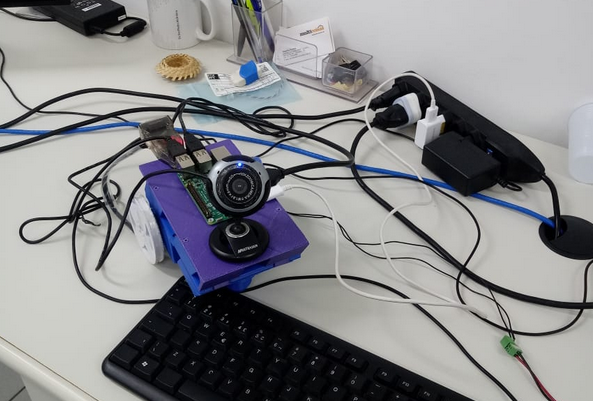
\includegraphics[scale=0.75, angle=0]{Figures/testefinal.png}
	\caption{Mockup de integração}
	\label{fig:testefinal}
	\source{Autores, 2019}
\end{figure}


